% This is LLNCS.DEM the demonstration file of
% the LaTeX macro package from Springer-Verlag
% for Lecture Notes in Computer Science,
% version 2.4 for LaTeX2e as of 16. April 2010
%
\documentclass{iacrtrans}
\usepackage{epstopdf}
\usepackage[T1]{fontenc}
\usepackage{lmodern}
\usepackage{relsize}
\usepackage[utf8]{inputenc}
\usepackage[compatibility=false]{caption}
\usepackage{subcaption}
\usepackage{pgf}
\usepackage{tikz}
\usetikzlibrary{arrows,automata}
\usepackage{tikz-timing}
\usepackage{todonotes}
\usepackage{tabularx}
\usepackage{microtype}
\usepackage{booktabs}
\usepackage{amsmath}
\usepackage{amssymb}
\usepackage{authblk}
\usepackage[hyphens]{url}
\usepackage{hyperref}
\hypersetup{breaklinks=true}
\usepackage{algorithm}
%\usepackage{algorithmic}
\usepackage{algpseudocode}
\usepackage{cite}
\usepackage{units}
%\usepackage{algpseudocode}
%\usepackage{algorithm2e}
%\usepackage[]{algorithm2e}
\usepackage{algpseudocode}
\usepackage{bm}
\usepackage{mathtools}
\usepackage{theorem}
\usepackage{mathrsfs}
\usepackage{listings}
\usepackage{cleveref}
\usepackage{pifont}
%\usepackage{refcheck}
\algnewcommand{\AND}{\algorithmicand}
\newcommand{\cmark}{\ding{51}}
\newcommand{\xmark}{\ding{55}}
\newcommand\numberthis{\addtocounter{equation}{1}\tag{\theequation}}
\newcommand{\eqd}{\ensuremath{=_{\mathrm{\scriptscriptstyle def}}}}
\newcommand{\Z}{\ensuremath{\mathbb Z}}
\newcommand\myE[1]{\ensuremath\mathbb{E}\left\lbrack #1 \right\rbrack} % The expectation (or mean, or esperance)
\newcommand\myV[1]{\ensuremath\mathsf{Var}\left\lbrack #1 \right\rbrack} % The variance
\newcolumntype{P}[1]{>{\centering\arraybackslash}p{#1}}
\setcounter{secnumdepth}{3}


\newcommand{\stodo}[1]{\todo[inline,caption={}]{TODO: #1}}
\newcommand{\minus}{\scalebox{0.75}[1.0]{$-$}}


%\newtheorem{theorem}{Theorem}
%\newtheorem{corollary}[theorem]{Corollary}
%\newtheorem{definition}[theorem]{Definition}
%\newtheorem{property}[theorem]{Property}
%\newtheorem{lemma}[theorem]{Lemma}

%%%% Special environments
%\newenvironment{proof}{\noindent \textbf{Proof}}{\qed \vskip 1em}
%\newcommand{\qed}{\hfill \ensuremath{\Box}}

%
\begin{document}
%

\title{Standard Lattice-Based Key Encapsulation\\ on Embedded Devices}

\author{
James Howe\textsuperscript{1}, Tobias Oder\textsuperscript{2}, Markus Krausz\textsuperscript{2}, and Tim G\"uneysu\textsuperscript{2,3}
}

\institute{
\textsuperscript{1}Department of Computer Science, University of Bristol, UK \texttt{james.howe@bristol.ac.uk}\\
\textsuperscript{2}Horst G\"ortz Institute for IT Security, Ruhr-Universit\"at Bochum, Germany \texttt{\{tobias.oder,markus.krausz,tim.gueneysu\}@rub.de}\\
\textsuperscript{3}DFKI, Germany\\
}

\keywords{Post-quantum cryptography, standard lattices, Frodo, KEM, FPGA, microcontroller, embedded security, hardware security.}

\maketitle

\begin{abstract} \label{abtract}
Lattice-based cryptography is one of the most promising candidates being considered to replace current public-key systems in the era of quantum computing. In 2016, Bos et al. proposed the key exchange scheme \textsf{FrodoCCS}, that is also a submission to the NIST post-quantum standardization process, modified as a key encapsulation mechanism (\textsf{FrodoKEM}). The security of the scheme is based on standard lattices and the learning with errors problem. Due to the large parameters, standard lattice-based schemes have long been considered impractical on embedded devices. The \textsf{FrodoKEM} proposal actually comes with parameters that bring standard lattice-based cryptography within reach of being feasible on constrained devices. In this work, we take the final step of efficiently implementing the scheme on a low-cost FPGA and microcontroller devices and thus making conservative post-quantum cryptography practical on small devices. 
Our FPGA implementation of the decapsulation (the computationally most expensive operation) needs 7,220 look-up tables (LUTs), 3,549 flip-flops (FFs), a single DSP, and only 16 block RAM modules. The maximum clock frequency is 162 MHz and it takes 20.7 ms for the execution of the decapsulation. Our microcontroller implementation has a 66\% reduced peak stack usage in comparison to the reference implementation and needs 266 ms for key pair generation, 284 ms for encapsulation, and 286 ms for decapsulation. Our results contribute to the practical evaluation of a post-quantum standardization candidate.
\end{abstract}
\input{tex/intro}
\input{tex/background}
\input{tex/hw_impl}
\section{Microcontroller Design}

We present four implementations of \textsf{FrodoKEM}. We implemented both parameter sets \textsf{FrodoKEM-640} and \textsf{FrodoKEM-976}
and we also implemented both possible pseudo-random numbers generators for the generation of $\mathbf{A}$. For AES, we rely on the optimized implementation by Schwabe and Stoffelen \cite{DBLP:conf/sacrypt/SchwabeS16} and for cSHAKE we use the assembly implementation from the official KECCAK code package \cite{bertoni2016keccak}.

\subsection{Target Platform}

We evaluate our microcontroller implementation of \textsf{FrodoKEM} on the STM32F407 Discovery board that has a 32-bit ARM Cortex-M4F microprocessor that runs with up to 168 MHz. Our development board comes with 192 kilobyte of RAM and one megabyte of Flash memory. Furthermore the Cortex-M4 features powerful DSP instructions like single-cycle multiply-with-accumulate and a true random number generator based on analog noise. However, in contrast to other M4-based microcontrollers, our development board does not have an AES-accelerator that could be used to speed-up \textsf{FrodoKEM-AES}. As development environment we use CooCox CoIDE version 1.7.7 with gcc-arm-none-eabi 5.4 2016 toolchain. The Cortex-M4F has 13 general purpose registers and ($R0-R12$), one register reserved for the stack pointer, a link register, one register reserved for the program counter, and special-purpose program status registers. When mixing C with assembly it is important to note that the calling convention requires parameters to be in $R0-R3$ and the result to be in $R0-R1$. The link register can be used as general purpose register as well, if the assembly function does not call any other function and its original value is restored before leaving the function.

\subsection{High-level Memory Optimization}

The official specification of \textsf{FrodoKEM} reports a peak stack memory usage of 189,176 bytes for \textsf{FrodoKEM-976-AES}. As our microcontroller has only access to 192 kilobytes of RAM, we carefully analyze the memory allocation of the reference implementation to see whether we can make the implementation more efficient in terms of memory usage. Keep in mind that for many applications there is another software running beside the KEM, therefore it is sensible to reduce the memory consumption as much as possible without sacrificing performance. With the help of the flow chart of the most important operations in \textsf{FrodoKEM} (Figure \ref{fig:flowchart_encaps} and \ref{fig:flowchart_decaps}), it is easily possible to see which matrices are used for which computations. The highlighted intermediate values are large arrays with $n \times \bar{n}$ elements. As we store each element in two bytes, this means that one large array requires $976 \times 8 \times 2 = 15,616$ bytes of RAM for each large array for \textsf{FrodoKEM-976-AES}. The non-highlighted intermediate values are small ($\bar{n} \times \bar{n}$ elements, i.e. 128 bytes) and therefore we focus on optimizing the large ones. 

The first thing to note about decapsulation, as shown in Figure \ref{fig:flowchart_decaps}, is that we need memory for at least two large arrays. For instance, during the computation of $\mathbf{B}''$, both inputs $\mathbf{E'}$ and $\mathbf{S'}$ are large. While $\mathbf{E'}$ can be generated on the fly, $\mathbf{S'}$ is loaded multiple times during the multiplication by $\mathbf{A}$ and therefore on-the-fly computation would imply regenerating the same value over and over again. Therefore we decided that the better trade-off would be to keep storage space for at least two large arrays. Another thing to note is that the right-hand side can be computed completely independent from the left-hand side. Therefore we can store $\mathbf{S'}$ in one of our two memory slots for large arrays and compute $\mathbf{V}$ and $\mathbf{B''}$ using the other memory slot. Once $\mathbf{V}$ and $\mathbf{B''}$ are calculated, $\mathbf{S'}$ is no longer used and can be replaced by $\mathbf{B'}$.

In the flow chart of encapsulation in Figure \ref{fig:flowchart_encaps} we can see that two large arrays are also sufficient for the encapsulation as the sampling of $\mathbf{E'}$ and the unpacking of $\mathbf{B}$ can be done on-the-fly. In fact the encapsulation needs even less memory as for instance the packing of $\mathbf{B'}$ could be done on-the-fly as well. But as the bottleneck in terms of memory consumption is the decapsulation, we do not further optimize the encapsulation.

\begin{figure*}[tbhp]
\centering

\includegraphics[scale=0.6]{figures/frodo_flowchart_encaps}

\caption{Flowchart of the encapsulation. Yellow highlighted matrices are $n \times \bar{n}$ matrices.}
\label{fig:flowchart_encaps}
\end{figure*}

\begin{figure*}[tbhp]
\centering

\includegraphics[scale=0.6]{figures/frodo_flowchart_decaps}

\caption{Flowchart of the decapsulation. Yellow highlighted matrices are $n \times \bar{n}$ matrices.}
\label{fig:flowchart_decaps}
\end{figure*}

\subsection{Low-level Assembly Optimization}

Our measurements indicate that besides the generation of the matrix $\mathbf{A}$, the multiplication of $\mathbf{A}$ with the secret matrix consumes most of the cycles, and therefore optimizing the multiplication is profitable. The simple operation of multiplication consumes just a small part of the cycles, the loading and storing of the matrix entries is the decisive part. Therefore minimizing the memory accesses is the key to a short run-time. Since the generation of the matrix $\mathbf{A}$ needs to be computed on-the-fly due to the memory constraints on the ARM Cortex-M4F, the multiplication cannot be done on the whole matrix $\mathbf{A}$ at once. We chose to generate $\mathbf{A}$ row-by-row when computing $\mathbf{AS}$. For the computation of $\mathbf{S'A}$ the generation of $\mathbf{A}$ depends on the choice of the permutation function. Writing the multiplication in assembly language gives us more control over the implementation and allows us to incorporate enhancements the compiler cannot engineer. Since the amount of memory accesses is substantial for the speed, our goal is to load the necessary matrix entries from RAM as rarely as possible and use all the available registers.

When $\mathbf{A}$ is generated on-the-fly, a straightforward implementation of the multiplication of $\mathbf{AS}$ has two loops. The first loop iterates over the columns of $\mathbf{S}$ with $\bar{n}$ iterations. The second loop iterates over the rows of $\mathbf{S}$, respectively the entries of the generated row of $\mathbf{A}$ with $n$ iterations.  But as $\bar{n} = 8$ in both parameter sets, it is possible to implement the matrix multiplication by using only one loop. During the multiplication of one row of $\mathbf{A}$ with $\mathbf{S}$, only eight entries of $\mathbf{AS}$ are computed. Since these entries are the sum of the products of $n$ multiplications, they are often updated during the computation. Storing the eight entries of $\mathbf{AS}$ in registers during the whole computation enables us to save many memory accesses: instead of iterating over the eight columns of $\mathbf{S}$, it is possible to process one entry of $\mathbf{A}$ with a complete row from $\mathbf{S}$ during one iteration. Figure \ref{fig:mul} presents this concept graphically.

  \begin{figure}[tbhp]
  	\centering
  	\includegraphics[width=1\textwidth,]{figures/mul.pdf}
  	\caption{Concept of the multiplication of one row of $\mathbf{A}$ with $\mathbf{S}$ effectively. Blue entries are affected by one function call, red entries are loaded during one iteration.}
  	\label{fig:mul}
  \end{figure}

The multiplication of $\mathbf{A}$ and matrix $\mathbf{S'}$ is slightly different, and variates with the use of either AES or cSHAKE. With cSHAKE, the matrix $\mathbf{A}$ is intended to be generated only in entire rows, which is convenient for the computation of $\mathbf{AS}$, but inefficient for the computation of $\mathbf{S'A}$, because one row of $\mathbf{A}$ affects all elements of $\mathbf{S'A}$. 
With AES, $\mathbf{A}$ is generated in blocks of 128 bits, therefore it is not only possible to generate $\mathbf{A}$ row-by-row but also by producing eight columns at a time. In a straightforward implementation, this leads to a third  loop iterating over the eight columns. The fact that the number of processed columns of $\mathbf{A}$ is eight, just as the parameter $\bar{n}$, enables us to use the same concept that we used for the multiplication of $\mathbf{S'A}$. We illustrate this concept in Figure \ref{fig:mulcol}. To avoid nested loops, we unroll the loop that gets added due to the eight columns. We end up with eight loops that are run through \emph{after} each other.
	
 \begin{figure}[tbhp]
   	\centering
   	\includegraphics[width=1\textwidth,]{figures/colmul.pdf}
   	\caption{Concept of the multiplication of 8 columns of $\mathbf{A}$ with $\mathbf{S'}$ effectively. Blue and light blue entries are affected by one function call, light blue entries are loaded by one entire loop, red entries are loaded during one iteration.}
   	\label{fig:mulcol}
 \end{figure}

The ARM Cortex-M4F offers 13 general purpose registers $R0-R12$ which we use all in our assembly matrix multiplication to maximize memory efficiency. Furthermore we use the designated link register $R14$ whose content we preserve on the stack. In $R0$ a pointer to matrix $\mathbf{A}$ is passed, in $R1$ a pointer to matrix $\mathbf{S}$, and in $R2$ a pointer to matrix $\mathbf{B}$. After loading the eight relevant entries of $\mathbf{B}$ into the registers $R4-R11$, we use $R2$ to store elements of $\mathbf{A}$. In $R3$ we pass the parameter $n$, which defines the number of iterations through the loop. In $R12$ and $R14$ entries of $\mathbf{S}$ are stored.

In both parameter sets, entries of matrices are stored in 16-bit data types, but the ARM Cortex-M4F is a 32-bit architecture. This enables us to reduce memory access, by loading two entries of matrix $\mathbf{A}$ simultaneously, as in Line 1 of Listing \ref{lst:loop1}. In the next line we use an instruction to load multiple aligned words, to get four entries of $\mathbf{S}$ by only one instruction. The single-cycle multiply-with-accumulate capabilities are very valuable for the actual matrix multiplication, used for example in Line 3 of Listing \ref{lst:loop1}.

\begin{lstlisting}[caption={Multiplication in Assembly}\label{lst:loop1}]
ldr r2, [r0], #4     //r2=a_ij+1, a_ij
ldmia r1!, {r12,r14} //r12=s_ij+1, s_ij, r14=s_ij+3,s_ij+2
mla r4, r2, r12, r4  //r4=r2*r12+r4
lsr r12, r12, #16    //r12=s_ij+1
mla r5, r2, r12, r5
mla r6, r2, r14, r6
lsr r14, r14, #16
mla r7, r2, r14, r7
\end{lstlisting}

\subsection{Protection Against Timing Side Channels}
Our implementations using cSHAKE have a constant timing and are therefore protected against timing attacks. The AES implementation from \cite{DBLP:conf/sacrypt/SchwabeS16} is very efficient but due to the caches on our development board not timing-constant. Therefore we disabled the data and instruction cache by clearing bit 9 and bit 10 of the \texttt{FLASH\_ACR} register. We noticed only a negligible drop in performance ($< 1$\%) after disabling the caches.

\section{Results and Comparison}
In this section we discuss the results of our FPGA and microcontroller implementations and compare our implementations with others. In particular, we also compare with implementations of \textsf{NewHopeUSENIX}, even though comparing a standard lattice-based scheme with an ideal lattice-based scheme is not exactly an apples-to-apples comparison (as discussed in Section \ref{sec:ringvsstandard}). Our intention behind this comparison is to show the cost of removing the potential additional attack vector of ideal lattices (i.e., the ring structure).
\subsection{FPGA Results}

%\begin{table}[tbhp]
%\caption{Resource consumption of \textsf{FrodoKEM-cSHAKE} on a Xilinx Artix-7 XC7A35T FPGA.}
%\label{tab:res_fpga}
%\begin{center}
%\begin{tabular}{|c|c|c|c|c|c|c|}
%\hline
%%& \multicolumn{2}{c|}{\textsf{FrodoKEM-AES}} &\multicolumn{2}{c|}{\textsf{FrodoKEM-cSHAKE}} &&\\
%\textsf{FrodoKEM} Operation	& LUT/FF & Slice & DSP & BRAM & MHz & Ops/sec\\
%\hline
%\textsf{FrodoKEM-640} Keypair	& 6621/3511 & 1845 & 1 & 6 & 167 & 51 \\
%\textsf{FrodoKEM-640} Encaps	& 6745/3528 & 1855 & 1 & 11 & 167 & 51 \\
%\textsf{FrodoKEM-640} Decaps	& 7220/3549  & 1992  & 1 & 16 & 162 & 49 \\ \hline
%\textsf{FrodoKEM-976} Keypair	& 7155/3528 & 1981 & 1 & 8 & 167 & 22 \\
%\textsf{FrodoKEM-976} Encaps	& 7209/3537 & 1985 & 1 & 16 & 167 & 22 \\
%\textsf{FrodoKEM-976} Decaps	& 7773/3559 & 2158 & 1 & 24 & 162 & 21 \\ %\hline\hline
%%\textsf{NewHope-1024} Server \cite{oder2017implementing}	& 5142/4452 & - & 2 & 4 & 125 & 731 \\
%%\textsf{NewHope-1024} Client \cite{oder2017implementing}	& 4498/4635 & - & 2 & 4 & 117 & 653 \\ \hline
%%\textsf{LWE} Encryption \cite{HoweMORGB16_1} & 6078/4676 & 1811 & 1 & 73 & 125 & 1272 \\
%\hline
%\end{tabular}
%\end{center}
%\end{table}

Table \ref{tab:comp_fpga} provides post-place and route results of the proposed hardware designs, as well as comparative lattice-based cryptographic hardware designs. The 18Kb BRAM usage follows the requirements of the inputs of the operations, those being the public-key, the secret-key, and the ciphertext information. The increased of BRAM usage in Decaps results in a slight decrease in clock frequency. The area consumption of all the modules are similar, at least for each parameter set. This is essentially due to the reuse of the LWE multiplication core, which is reused for all vector-matrix multiplication and error addition operations. The increase between parameter sets is due to an increase from 640 to 976 in the matrix dimension, the rest of the design essentially remains the same.


\begin{table}[tbhp]
\caption{FPGA resource consumption of the proposed \textsf{FrodoKEM-cSHAKE} hardware design, with its sub-modules ($^*$), alongside \textsf{NewHopeUSENIX-1024} \cite{oder2017implementing} and \textsf{Standard-LWE} encryption \cite{DBLP:conf/dac/HoweMORGB16} hardware designs for comparison. \textsf{FrodoKEM} and \textsf{NewHopeUSENIX-1024} utilize a Xilinx Artix-7 FPGA and \textsf{Standard-LWE} utilizes a Xilinx Spartan-6 FPGA.}
\label{tab:comp_fpga}
\begin{center}
\resizebox{\textwidth}{!}{
\noindent\makebox[\textwidth]{
\begin{tabular}{|c|c|c|c|c|c|c|}
\hline
%& \multicolumn{2}{c|}{\textsf{FrodoKEM-AES}} &\multicolumn{2}{c|}{\textsf{FrodoKEM-cSHAKE}} &&\\
Cryptographic Operation	& LUT/FF & Slice & DSP & BRAM & MHz & Ops/sec\\
\hline
\textsf{FrodoKEM-640} Keypair 	& 6621/3511 & 1845 & 1 & 6 & 167 & 51 \\
\textsf{FrodoKEM-640} Encaps	& 6745/3528 & 1855 & 1 & 11 & 167 & 51 \\
\textsf{FrodoKEM-640} Decaps	& 7220/3549  & 1992  & 1 & 16 & 162 & 49 \\ \hline
\textsf{FrodoKEM-976} Keypair	& 7155/3528 & 1981 & 1 & 8 & 167 & 22 \\
\textsf{FrodoKEM-976} Encaps	& 7209/3537 & 1985 & 1 & 16 & 167 & 22 \\
\textsf{FrodoKEM-976} Decaps	& 7773/3559 & 2158 & 1 & 24 & 162 & 21 \\ \hline
cSHAKE$^*$	& 2744/1685 & 766 & 0 & 0 & 172 & 1.2m \\
Error+AES Sampler$^*$ & 1901/1140 & 756 & 0 & 0 & 184 & 184m \\

\hline\hline
\textsf{NewHopeUSENIX} Server \cite{oder2017implementing} 	& 5142/4452 & 1708 & 2 & 4 & 125 & 731 \\
\textsf{NewHopeUSENIX} Client \cite{oder2017implementing}	& 4498/4635 & 1483 & 2 & 4 & 117 & 653 \\ \hline
\textsf{LWE} Encryption \cite{DBLP:conf/dac/HoweMORGB16}  & 6078/4676 & 1811 & 1 & 73 & 125 & 1272 \\
\hline
\end{tabular}}}
\end{center}
\end{table}

Hardware results are also provided for the main components required; the error distribution sampler and the cSHAKE module. As per the specifications, the error sampler is combined with AES as a PRNG input to the lookup table. The large area consumption of this module is due to the use of AES, as well as employing a large number of comparators in order for high throughput. One cSHAKE module is used for generating the randomness for the matrix $\mathbf{A}$ and a second is used to generate the shared secret $\mathbf{ss}$ on-the-fly, which makes these cSHAKE modules the largest overall. The remaining area usage is consumed by control logic and the LWE multiplier; which requires a DSP for multiplication and a reasonable amount of LUTs for storage.


In Table \ref{tab:clks_fpga} we present the cycle counts for our FPGA designs. Clock cycle counts in Table \ref{tab:clks_fpga} are equivalent for the PRNG choice (either AES or cSHAKE) as this module runs in parallel to the vector-matrix multiplication within the LWE multiplication core, and does not affect the critical path of the operations (as described in Section \ref{sec:lwe_core}). The clock cycle counts for each cryptographic operation are defined by the MAC operations of all the matrix-matrix multiplications they require. Moreover, the multiplication of the largest matrices in each cryptographic operation, that is; $\mathbf{B} \leftarrow \mathbf{A} \mathbf{S} + \mathbf{E}$ for key generation, $\mathbf{B}^\prime \leftarrow \mathbf{S}^\prime \mathbf{A} + \mathbf{E}^\prime$ for encapsulation, or $\mathbf{B}^{\prime\prime} \leftarrow \mathbf{S}^\prime \mathbf{A} + \mathbf{E}^\prime$ for decapsulation, respectively contribute 100\%, 97.5\%, and 97.5\% to their overall clock cycle counts. As described in Section \ref{sec:frodo_fpga}, there is a one-time initialisation stage, for loading input information, initialising modules, and pre-storage matrices. This process lasts between 5.1k and 23.5k clock cycles, depending on the operation and parameter set used. This extra latency is not included in Table \ref{tab:clks_fpga} as it is negligible, even for one run of a \textsf{FrodoKEM} operation (at most, $< 0.5 \%$), and becomes even more so when averaged over numerous operations.

%For example in \textsf{FrodoKEM-640} encaps, this stage requires 5.1k clock cycles to load key information

\begin{table}[tbhp]
\caption{Clock cycle counts for our FPGA implementations of \textsf{FrodoKEM}.}
\label{tab:clks_fpga}
\begin{center}
\begin{tabular}{|l|r|r|r|r|}
\hline
& \multicolumn{2}{c|}{\textsf{FrodoKEM-AES}} &\multicolumn{2}{c|}{\textsf{FrodoKEM-cSHAKE}} \\
Operation	  & $n=640$ & $n=976$ & $n=640$ & $n=976$\\
\hline
%Operation 1					& xxx & xxx & xxx & xxx \\
%Operation 2					& xxx & xxx & xxx & xxx \\
%Operation 3					& xxx & xxx & xxx & xxx \\
Keypair							& 3,276,800 & 7,620,608 & 3,276,800 & 7,620,608 \\
Encaps							& 3,317,760 & 7,683,072 & 3,317,760 & 7,683,072 \\
Decaps							& 3,358,720 & 7,745,536 & 3,358,720 & 7,745,536 \\
\hline
\end{tabular}
\end{center}
\end{table}

Comparison results for related works is given in Table \ref{tab:comp_fpga}. The FPGA device used, the Xilinx Artix-7 XC7A35T FPGA, is similar to the one used by Oder and G{\"u}neysu \cite{oder2017implementing}, in order for a fair comparison. Although the \textsf{NewHopeUSENIX} design outperforms our proposed designs in terms of operations per second, the area consumption is comparable. The loss in throughput is expected and almost entirely due to the number of clock cycles required for each operation; \textsf{NewHopeUSENIX} requires 171k clock cycles for the server-side operations whereas \textsf{FrodoKEM} requires 3.3m. The increase in memory requirements is due to the differences in the key sizes, since \textsf{NewHopeUSENIX} uses polynomials instead of the matrices used in \textsf{FrodoKEM} (as mentioned in Section \ref{sec:ringvsstandard}).

The only other implementation of standard lattice-based cryptography in hardware is by Howe et al. \cite{DBLP:conf/dac/HoweMORGB16}, referred to as \textsf{Standard-LWE}, and is discussed here for comparison. The area consumptions are similar due to the similar LWE multiplication operations required, however, Howe et al. uses significantly smaller matrix dimensions in comparison to the \textsf{FrodoKEM} parameters, and hence we see an improvement. Moreover, their use of BRAM is significantly larger, due to precomputed keys, which we mitigate by using on-the-fly generation. Reusing keys is discussed by the authors of \textsf{FrodoKEM} \cite[Sec. 5.1.4]{frodo-nist} but is not recommended due to the potential attack vector it provides. Additionally, we also wanted to keep the memory requirements low and therefore decided to not store the entire matrix $\mathbf{A}$ in memory. The throughput performance of \textsf{Standard-LWE} is much higher in comparison to our research, due to a much lower clock cycle count of 98k required. This is essentially due to, again, the significantly smaller matrix dimensions and hence less multiplications required. Comparing the overall security targets of the schemes shows that the \textsf{Standard-LWE} implementation only provides 128 bits of \textit{classical} security, whereas our implementations provide 128 and 192 bits of post-quantum security.

%\textsf{Stanard-LWE} achieves such a low clock cycle count because the matrix $\mathbf{A}$ is precomputed and stored in memory, whereas in our implementation $\mathbf{A}$ is generated on-the-fly and clearly the bottleneck. 



\subsection{Microcontroller Results}
We use the pqm4 framework \cite{pqm4} to evaluate the proposed microcontroller implementation. In the framework, the running time of an operation is measured in cycle counts using libopencm3\footnote{\url{http://libopencm3.org/}}. The framework can also measure the stack usage with the help of stack canaries. Our development board runs at a clock frequency of 168 MHz.

In Table \ref{tab:res_micro} we show the cycle counts for the major building blocks of \textsf{FrodoKEM} as well as the entire key pair generation, encapsulation, and decapsulation. At 168 MHz, the key generation takes 266 ms, the encapsulation takes 284 ms, and the decapsulation takes 286 ms for \textsf{FrodoKEM-640-AES}. For \textsf{FrodoKEM-940-AES} the cycle counts are more than twice as high as for \textsf{FrodoKEM-640-AES}. The main reason for that is that the size of the matrix $\mathbf{A}$ grows quadratically when $n$ grows and the generation of $\mathbf{A}$ is the most time consuming part of our implementation. Further speed-ups could be achieved by speeding up the AES implementation. However, to the best of our knowledge, the implementation by Schwabe and Stoffelen \cite{DBLP:conf/sacrypt/SchwabeS16} that we used in our implementation is already the fastest published AES implementation. Some Cortex-M4-based microcontrollers also have access to an on-board hardware AES engine that would further speed up the AES. The implementations of \textsf{FrodoKEM-cSHAKE} are slower than \textsf{FrodoKEM-AES} implementations as cSHAKE is based on KECCAK and hardware platforms are where KECCAK really excels on, not software \cite{SHA3}. Therefore we expected \textsf{FrodoKEM-cSHAKE} to have a worse performance than \textsf{FrodoKEM-AES}.  

We furthermore see in Table \ref{tab:res_micro} that the $\mathbf{AS} + \mathbf{E}$ is the most time consuming part of the key pair generation as it accounts for 93\% of the run time for \textsf{FrodoKEM-640-AES}. Similarly $\mathbf{S}^\prime \mathbf{A} + \mathbf{E}^\prime$ is bottleneck for encapsulation and decapsulation (88\% resp. 87\%). The second most time-consuming operation is the sampling of a noise matrix. We measured the performance of noise sampling for matrices with dimension $n \times \bar{n}$. This operation is performed twice during every run of key pair generation, encapsulation, and decapsulation. It accounts for 6\% of the run time of each of the three algorithms (\textsf{FrodoKEM-640-AES}). In comparison to the computation of $\mathbf{AS} + \mathbf{E}$ or $\mathbf{S}^\prime \mathbf{A} + \mathbf{E}^\prime$, multiplications of smaller matrices cost much less cycles, as one can see in the cycle counts for $\mathbf{S}^\prime \mathbf{B} + \mathbf{E}^{\prime\prime}$.

\begin{table}[tbhp]
\caption{Cycle counts for our microcontroller implementation measured at a clock frequency of 168 Mhz.}
\label{tab:res_micro}
\begin{center}
\begin{tabular}{|l|r|r|r|r|}
\hline
& \multicolumn{2}{c|}{\textsf{FrodoKEM-AES}} &\multicolumn{2}{c|}{\textsf{FrodoKEM-cSHAKE}} \\
Operation	  & $n=640$ & $n=976$ & $n=640$ & $n=976$\\
\hline
$\mathbf{S}^\prime \mathbf{B} + \mathbf{E}^{\prime\prime}$	& 451,442  		& 687,728  		& 451,442  		& 687,728  \\
$\text{SampleMatrix}(\cdot,n,\bar{n},\cdot,\cdot)$					& 1,344,962  	& 1,480,483  	& 1,344,963  	& 1,480,484  \\
$\mathbf{AS} + \mathbf{E}$																	& 41,308,745 	& 96,035,515  & 82,256,529  & 181,809,613  \\
$\mathbf{S}^\prime \mathbf{A} + \mathbf{E}^\prime$					& 41,833,535  & 97,266,270  & 106,178,196 & 244,078,721  \\\hline
Keypair							& 44,603,160   & 101,273,066  & 85,585,315 & 187,070,653  \\
Encaps							& 47,742,966   & 106,933,956  & 112,103,350  & 253,735,550  \\
Decaps							& 48,051,929   & 107,393,295  & 112,442,770   & 254,194,895  \\
\hline
\end{tabular}
\end{center}
\end{table}

In Table \ref{tab:res_micro_mem} we list the peak stack usage for our implementations. For $n = 976$ the \textsf{FrodoKEM} specification \cite{frodo-nist} reports a peak stack memory usage of 189 kilobytes when using AES as PRNG and 156 kilobytes when using cSHAKE. The specification reports at most 81,836 bytes as static library size for non-vectorized implementations. As our development board has access to 192 kilobytes of RAM and one megabyte of Flash memory, the peak stack usage is what we focus on in the following. We managed to reduce these numbers so that the implementation comfortably fits onto the microcontroller and still leaves space for other applications running on it. For the AES-based implementation we reduced the memory consumption by 66\% and for the cSHAKE implementation we reduced it by 63\%.

\begin{table}[tbhp]
\caption{Stack usage in bytes for our microcontroller implementation.}
\label{tab:res_micro_mem}
\begin{center}
\begin{tabular}{|l|r|r|r|r|}
\hline
& \multicolumn{2}{c|}{\textsf{FrodoKEM-AES}} &\multicolumn{2}{c|}{\textsf{FrodoKEM-cSHAKE}} \\
Operation	  & $n=640$ & $n=976$ & $n=640$ & $n=976$\\
\hline
Keypair							& 23,396   & 35,484  & 22,376  & 33,800   \\
Encaps							& 41,292   & 63,484  & 37,792  & 57,968   \\
Decaps							& 51,684   & 63,628  & 48,184  & 58,112   \\
\hline
\end{tabular}
\end{center}
\end{table}


\begin{table}[tbhp]
\begin{center}
\caption{Comparison of our microcontroller implementation with other implementations.}
\label{tab:micro_comparison}
\begin{tabular}{|l|l|r|r|}
\hline
Implementation & Platform & Security Level & Cycle counts\\\hline
\textsf{FrodoKEM-976-AES} (\textbf{this work})	& Cortex-M4 & 192 bits  & 315,600,317\\
\textsf{FrodoKEM-640-cSHAKE} \cite{pqm4} & Cortex-M4 & 128 bits & 318,037,129 \\
\textsf{KyberNIST-768} \cite{pqm4} & Cortex-M4 & 192 bits & 4,224,704 \\
\textsf{NewHopeUSENIX-1024} \cite{alkim2016newhope}	& Cortex-M4 &255 bits & 2,561,438 \\
ECDH scalar multiplication \cite{DBLP:journals/dcc/DullHHHPSS15} &  Cortex-M0 & pre-quantum & 3,589,850\\
\hline
\end{tabular}
\end{center}
%\vspace{-0.7cm}
\end{table}

In Table \ref{tab:micro_comparison} we compare our implementation with other implementations of key exchange schemes on Cortex-M microprocessors. Our implementation of \textsf{FrodoKEM-976-AES} has a similar performance compared to the implementation of \textsf{FrodoKEM-640-cSHAKE} from the pqm4 library \cite{pqm4} even though the security level is higher (192 vs. 128 bits). Our implementation is two orders of magnitude slower than the \textsf{NewHopeUSENIX} implementation from \cite{alkim2016newhope}. The reason for that is that \textsf{NewHopeUSENIX} is based on ideal lattices that are inherently much more efficient as the main operation in ideal lattice-based cryptography is polynomial multiplication. Polynomial multiplication in integer rings can be efficiently realized with the number-theoretic transform that has a complexity of $O(n \log (n))$ while the matrix operations in \textsf{FrodoKEM} have a complexity of $O(n^2)$. Therefore a decently optimized implementation of a scheme based on ideal lattices will always be faster than any implementation of a scheme based on standard lattices targeting a similar security level. Furthermore, the implementation in \cite{alkim2016newhope} is only secure against chosen-plaintext attackers, not chosen-ciphertext attackers. Unsurprisingly the \textsf{KyberNIST-768} implementation from pqm4 also provides a better performance, as \textsf{KyberNIST-768} is a module lattice-based scheme that still retains some of the structure of ideal lattices and in particular also benefits from the speed-ups from the number-theoretic transform. The ECDH implementation of \cite{DBLP:journals/dcc/DullHHHPSS15} is also much more efficient. But as ECDH is not secure against attacks by quantum computers, it cannot be considered as alternative to \textsf{FrodoKEM}.

While being significantly slower than implementations of other schemes, \textsf{FrodoKEM} is also a very conservative choice that does not suffer from relying on a structured lattice as potential additional attack vector (like for instance \textsf{NewHopeUSENIX} does). Depending on the use case it might be sensible to use \textsf{NewHopeUSENIX} in scenarios that demand high efficiency and moderate security and use \textsf{FrodoKEM} in cases that have very high security requirements.
\input{tex/conclusions}

\section*{Acknowledgement}
This research was supported in part by the European Union Horizon 2020 SAFEcrypto project (grant no. 644729) and by EPSRC via grant EP/N011635/1. We would also like to thank the anonymous reviewers for their very valuable and helpful feedback.


\bibliographystyle{alpha}
\bibliography{paper,references}

\end{document}
